\section{Luminaire Parameters}
For the calculations one type of luminaire has been chosen. From a wide range of outdoor luminaire procuders and distributors at the Czech market the luminaire Atos of the Schr\'{e}der company has been chosen. Atos luminaires are nowadays widely used for public outdoor lighting and can be fitted with light sources from 50~W to 150~W, making it suitable for road lighting of lower categories, e.g. pedestrian zones, cycleways, emergency lanes etc.

The adjustment of luminous intensity distribution curves can be achieved by a displacement of the light source inside the luminaire. The luminaire Atos offers 12 positions of the light source inside the luminaire, therefore 12 different luminous intensity distribution curves can be obtained.

\begin{figure}[htb]
  \centering
  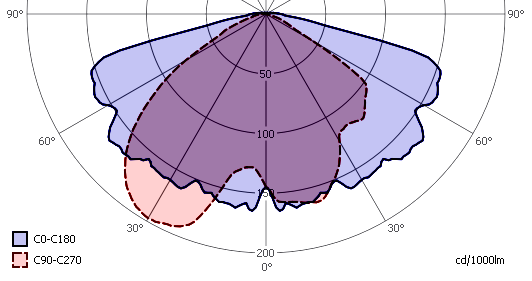
\includegraphics[width=\columnwidth]{70W_A1_v2}
  \caption{Luminous intensity distribution curves of ATOS/1627/SMOOTH POLYCARBONATE/SON-T 70/-17/100/10$^\circ$}
  \label{fig:lumIntDistr}
\end{figure}

